

The table \ref{table-spkshow-perf} shows the average $Fm$ per $SpkShow$ for the different systems.
\begin{table*}[t]
\begin{center}
\begin{tabular}{r||c|c|c|c}
& Percol & Qcompere & Soda & Oracle \\\hline\hline
average $Fm$ & 0.361 & 0.381 & 0.351 & 0.462\\\hline
average $Fm$ for in dictionary speakers & 0.628 & 0.684 & 0.619 & 0.722\\\hline
\#$SpkShow$ out of dictionary & 200 & 209 & 204 & 172\\\hline
\#$SpkShow$ in dictionary & 277& 268 & 273 & 305\\\hline
\#$SpkShow$ in dictionary, with $Fm=0$ & 79 & 63 & 86 & 63\\\hline
\end{tabular}
\caption{Average system performances per $SpkShow$}
\label{table-spkshow-perf}
\end{center}
\end{table*}

From the table we can notice the important number of $SpkShow$ which are not in the dictionary of the system, about 40\% for each system. As they don't have any model, they obviously cannot be identified, leading to an average global $Fm$ rather poor. More interestingly, the number of $SpkShow$ which are actually in the dictionary and which are not recognised at all, is not negligeable: their represent between 23.5\% to 31.5\% of the in-dictionary $SpkShow$, according to the systems.


Figure~\ref{fig:FMeasureDistribution} plot the distribution of all the $SpkShow$ in the system dictionaries, according their performance $Fm$, for the different systems. Foreach $Spkshow$, the average performance and the maximal performance obtained across systems are computed, and the corresponding distribution are also plotted. We can see from this figure that the average performance (from 61.9\% to 68.9\% according to the systems) presented in table\ref{table-spkshow-perf} is not at all representative of the performances obtained foreach $SpkShow$: speakers are either not recognized or well recognized. Indeed, if we compute the average performance for $SpkShow$ which have $Fm \neq 0$, the average $Fm$ grows to 87.9\% for PERCOL, 89.5\% for QCompere and 90.3\% for SODA. 

% \begin{figure}[!h]
% 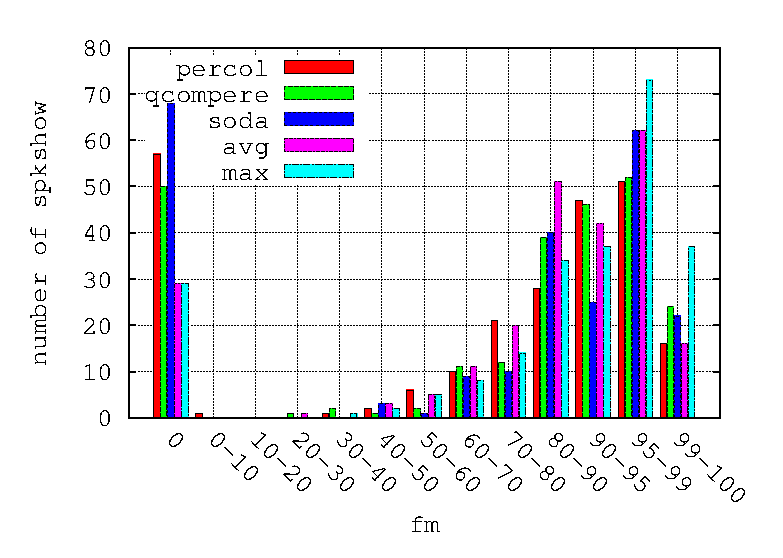
\includegraphics[scale=0.6]{figures/PQS-mono-model.eps}
% \caption{$spkShow$ performance distribution, for each system}
% \label{PQS}
% \end{figure}

To evaluate the impact of the automatic speaker diarization, we also perform the speaker analysis performance, for systems applied on reference speaker diarization. Results for systems PERCOL is shown in Figure~\ref{fig:autoVSref}.  
The comparison of the speaker identification performance between using the reference or automatic speaker diarization, carried out on PERCOL and SODA systems, shows that 38 $SpkShow$ (over the 277 in-dictionary speakers) for PERCOL and 14 $SpkShow$ (over the 273 in-dictionary speakers) for SODA present a null f-measure ($Fm_i=0$) with the automatic speaker diarization and a f-measure above 0.9 (above 0.97 for PERCOL and 0.92 for SODA) with the reference one. For these particular $SpkShow$, the quality of the automatic speaker diarization is the main reason of the poor speaker identification performance since a fine-grained analysis of the speaker diarization outputs highlighted segment frontier errors, clustering confusion errors, or both of them. The purity of the clusters, on which the automatic speaker identification process is applied, is incriminated here. 
In addition, we considered the $SpkShow$ for which a null f-measure is obtained whatever the speaker diarization implied. This observation was made for 41 $SpkShow$ with PERCOL system and 72 with SODA system, 12 $SpkShow$ being common to both of them. Focusing on $SpkShow$ for which more than 10s are available for speaker identification in the speaker diarization reference, the amount of training data available per $SpkShow$  could not explain the poor performance observed (mean duration of 649,77s, minimum and maximum values of 34.19s and 5277.52s for PERCOL, mean duration of 613.3s, minimum and maximum values of 145.5s and 714.76s for SODA). 
To be independent of the intrinsic quality of the speaker identification systems, we focused our attention on the 12 common $SpkShow$ mentioned above by studying the reference segments involved in the speaker identification process. The analysis revealed that these segments were associated with very poor acoustic quality : a large amount of overlapped speech for 4 $SpkShow$ (from 20 to 90\% of overlapped speech according to  $SpkShow$), an entire interview made by phone for 1 $SpkShow$, poor sound quality with reverberation for 1 $SpkShow$, and large background noise (street, assembly background voices, applause, etc) or music for 8 of them.

\begin{figure}[t]
\centering
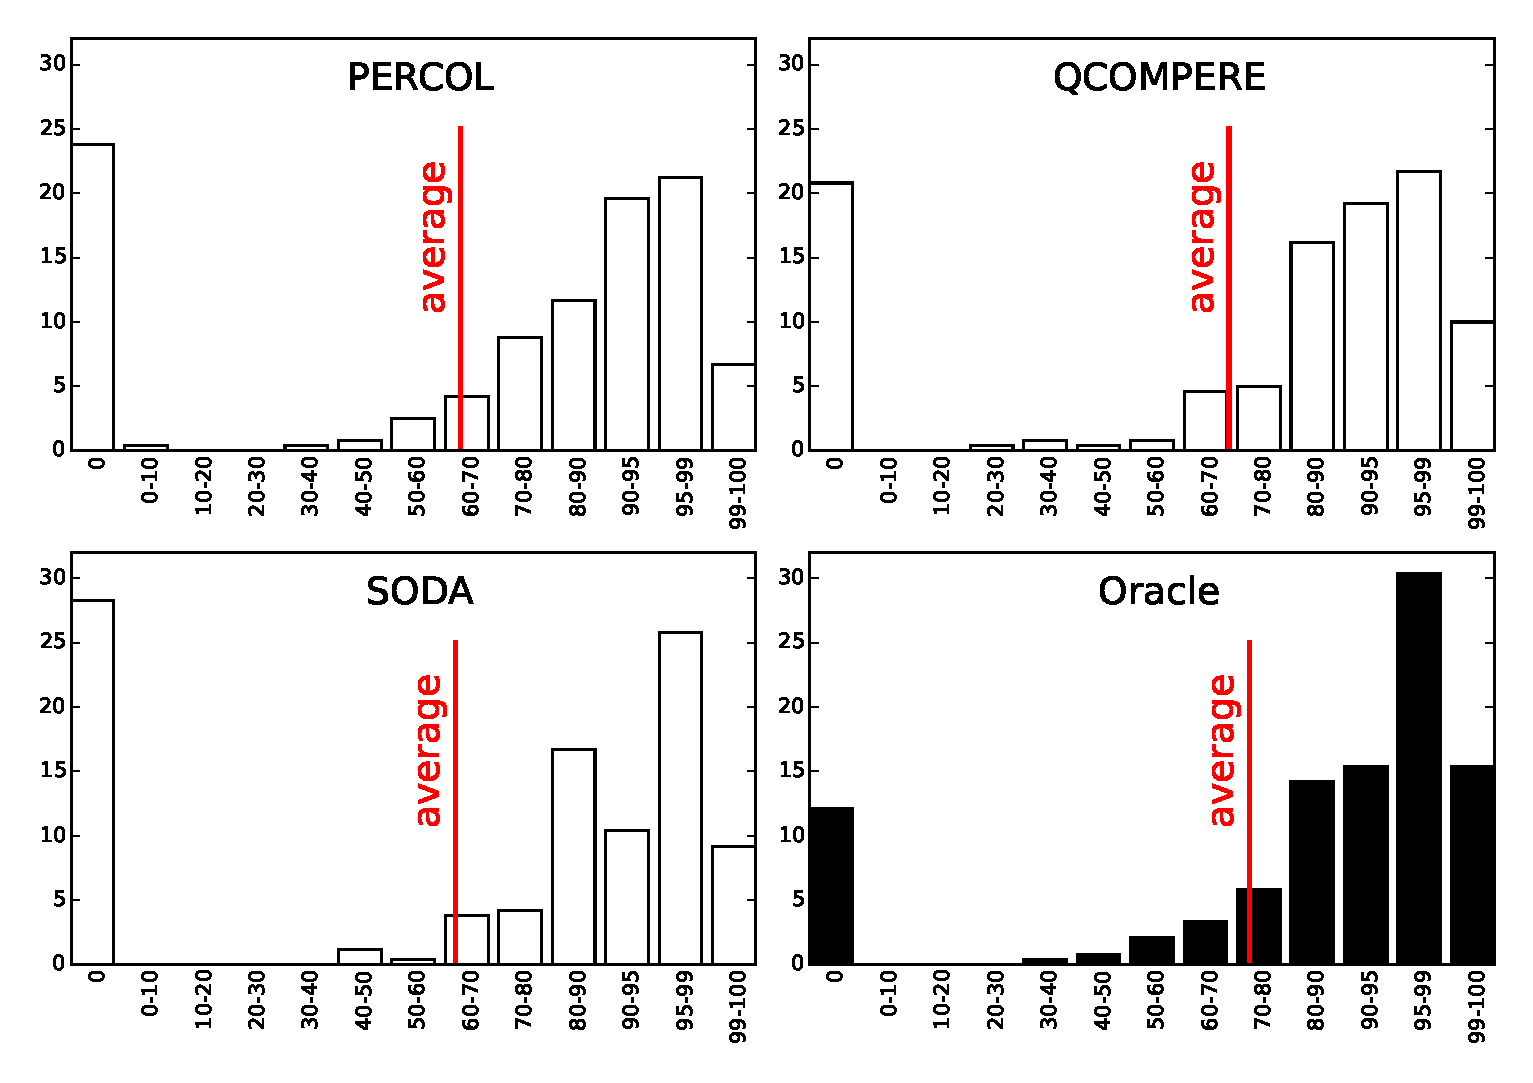
\includegraphics[width=\linewidth]{figures/bimodal.eps}
\caption{Distribution of $SpkShow$ according to system performance}
\label{fig:FMeasureDistribution}
\end{figure}


\begin{figure}[t]
\centering
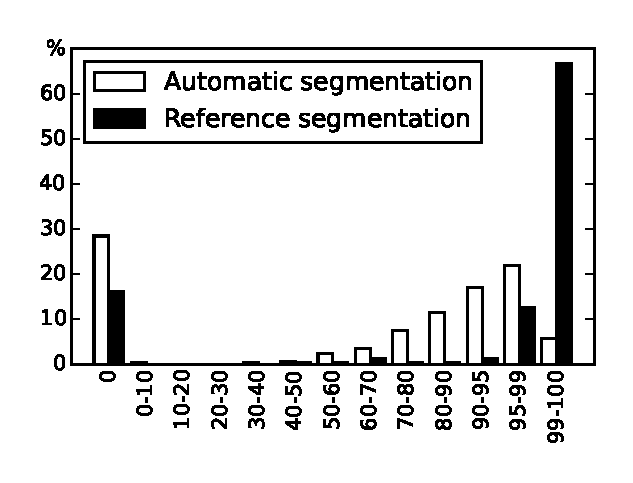
\includegraphics[width=\linewidth]{figures/ref.eps}
\caption{Effect of segmentation errors on PERCOL.}
\label{fig:autoVSref}
\end{figure}

